\documentclass{article}
\usepackage[utf8]{inputenc}

% Page setup
\usepackage[a4paper,landscape,margin=2cm]{geometry}
\usepackage{amsmath}

% Typography
\usepackage[scaled]{helvet}
\let\familydefault\sfdefault

\usepackage[usenames,svgnames]{xcolor}
\usepackage{tikz,pgfplots}
\usetikzlibrary{positioning,arrows,intersections}

\definecolor{colordict}     {RGB}{143,232,186}
\definecolor{colortext}     {RGB}{29 ,29 ,27 }
\definecolor{colordelta}    {RGB}{199,212,104}

\begin{document}
\pagestyle{empty}
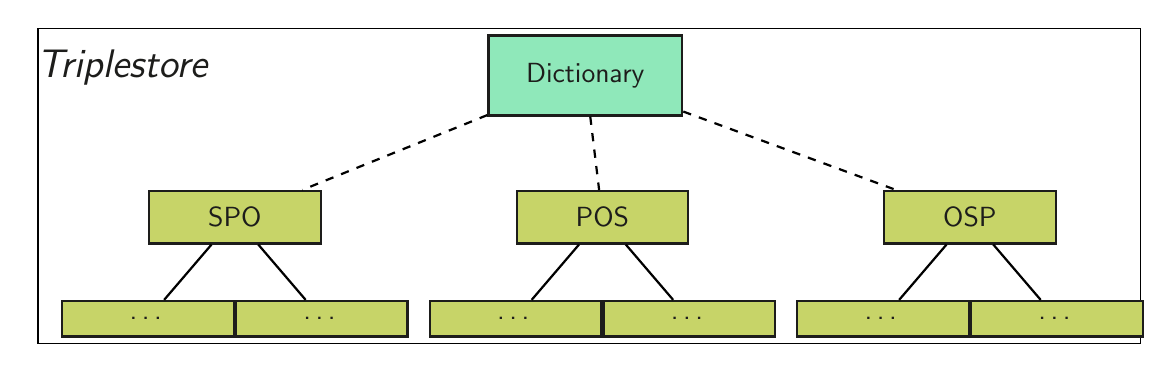
\begin{tikzpicture}[
    node distance = 7em, auto,
    font={\Large\itshape},
    title/.style={text=colortext,font={\Large\itshape}},
    code/.style={text=colortext,font={}},
    base/.style={text=colortext,font={},inner sep=6pt,align=center,rectangle},
    treenode/.style={base,thick,draw=colortext,text width=5em},
]

    \draw[] (0,0) rectangle (14,4);
    \node[title,text width=20em] at (3.5,3.5) {Triplestore};
    
    % Indexes
    \node[treenode,fill=colordelta] (asporoot) at (2.5,1.6)        {SPO};
    \node[treenode,fill=colordelta,below=of asporoot.south west,yshift=5em] (aspo1) {\ldots};
    \node[treenode,fill=colordelta,below=of asporoot.south east,yshift=5em] (aspo2) {\ldots};
    \draw[-,thick](aspo1) -- (asporoot);
    \draw[-,thick](aspo2) -- (asporoot);
    \node[treenode,fill=colordelta,right=of asporoot] (aposroot)        {POS};
    \node[treenode,fill=colordelta,below=of aposroot.south west,yshift=5em] (apos1) {\ldots};
    \node[treenode,fill=colordelta,below=of aposroot.south east,yshift=5em] (apos2) {\ldots};
    \draw[-,thick](apos1) -- (aposroot);
    \draw[-,thick](apos2) -- (aposroot);
    \node[treenode,fill=colordelta,right=of aposroot] (aosproot)        {OSP};
    \node[treenode,fill=colordelta,below=of aosproot.south west,yshift=5em] (aosp1) {\ldots};
    \node[treenode,fill=colordelta,below=of aosproot.south east,yshift=5em] (aosp2) {\ldots};
    \draw[-,thick](aosp1) -- (aosproot);
    \draw[-,thick](aosp2) -- (aosproot);
    
    % Dict
    \node[treenode,fill=colordict,inner sep=10pt] (dict) at (6.95,3.4) {Dictionary};
    \draw[-,thick,dashed](dict) -- (asporoot);
    \draw[-,thick,dashed](dict) -- (aposroot);
    \draw[-,thick,dashed](dict) -- (aosproot);
    

\end{tikzpicture}
\end{document}
